\chapter{Conceptos teóricos esenciales}\label{chapter:theoretical-framework}


En el presente capítulo se brinda una breve explicación de los conceptos del análisis de imágenes y la visión computacional tenidos en cuenta durante el desarrollo del trabajo. En la Sección \ref{section:rgbd} se presentan los principios de la tecnología RGB-D y el funcionamiento de las cámaras de profundidad, en particular la Intel\textregistered~RealSense\texttrademark~Depth Camera D435i. En la Sección \ref{section:imgEnh} se presentan los fundamentos básicos del procesamiento de imágenes empleados en la investigación. Por otro lado, en la Sección \ref{section:tracking} se explican los algoritmos de seguimiento de objetos en muestras de vídeo. Luego, en la Sección \ref{section:seg} se detallan los principios y algoritmos de segmentación en imágenes RGB. La Sección \ref{section:rec3d} aborda los algoritmos y etapas de la reconstrucción 3D utilizando imágenes de profundidad. Posteriormente, en la Sección \ref{section:measure} se sientan las bases de las mediciones de perímetro, área y volúmen de mallas en nubes de puntos 3D.

\section{Tecnología RGB-D}\label{section:rgbd}

La imagen es la estructura de datos más empleada en el campo de visión por computadoras o visión computacional. Una imagen permite almacenar una porción del entorno en un instante determinado.

\begin{definition}\label{def:img}
	Se define una imagen $I_{n \times m}$ como un arreglo bidimensional (matriz) con $n$~filas y $m$ columnas, tal que $I_{n \times m}[i, j] = p_{i,j}$ es un píxel y se cumple que $p_{i, j} \in \mathbb{N}^k: 0~\leq~i~\leq~n - 1 \wedge 0 \leq j \leq m - 1 \wedge k \in \mathbb{N}$.
\end{definition}

\begin{definition}
	El valor de $p_{i, j} \in \mathbb{N}^k$ se denomina intensidad o color del píxel en la posición $i, j$ de la imagen $I_{n \times m}$. El valor de $k$ (usualmente $1$ o $3$) varía en dependencia del espacio de color en el cual se tome la imagen u otras características adicionales que se asocien a cada píxel.
\end{definition}

A continuación se describen los espacios de color utilizados en la propuesta de software:

\begin{itemize}
	\item \textbf{RGB} es uno de los espacios de colores más populares utilizados para la representación de imágenes digitales. Está basado en la teoría tricromátrica~\footnote{La Teoría tricromática o de Young-Helmholtz establece que la mayoría de los colores se pueden igualar superponiendo tres fuentes de luz separadas o canales de colores utilizando el proceso de mezcla aditiva.} y por lo tanto define a cada color como una combinación de los tres colores primarios (rojo, verde y azul). Este espacio se define geométricamente como un cubo en donde cada coordenada puede tomar valores desde 0 hasta 255 (8 bits) \cite{sangwine1998colour}. Se considera que este espacio de color es dependiente del dispositivo con el que se capture la imagen \cite{tkalcic2003colour, ruela2013role}. En este espacio se tiene que $p_{i, j} = [R, G, B]$ por lo cual $k=3$ en la definición \ref{def:img}.
	
	\item \textbf{HSV} es una transformación de las coordenadas rectangulares de RGB a cilíndricas. En este espacio cilíndrico, cada color está representado por una combinación de matiz (H), saturación (S) y brillo (V). El matiz es la coordenada angular y varía de $0^{\circ}$ a $360^{\circ}$. La saturación es la cantidad de color puro presente en la región con respecto a la cantidad de blanco, esta varía entre cero y uno. Finalmente, el brillo, mide la cantidad de blanco presente en el color y varía de 0 a 255 \cite{ruela2013role}. Este espacio aporta igualmente tres componentes y $p_{i, j} = [H, S, V]$.
	
	\item \textbf{L*a*b} El espacio de color L*a*b* resulta de una transformación no lineal del espacio RGB \cite{bradski2000opencv}. L* representa el brillo, mientras a* y b* representan el matiz y la saturación de un color. En este espacio de color L* se desplaza de negro a blanco, mientras a* se desplaza desde verde a rojo y b* desde azul a amarillo. Este espacio aporta tres componentes y $p_{i, j} = [L, a, b]$.
	
	\item \textbf{YCbCr} Es una familia de espacios de color utilizadas en sistemas de vídeo. El valor de Y denota la luminancia, mientras Cb y Cr son las componentes de crominancia azul y roja respectivamente \cite{sergyan2007color}. Este espacio aporta tres componentes $p_{i, j} = [Y, Cb, Cr]$.
\end{itemize}

Una imagen presentada en cualquiera de los espacios anteriores brinda información del entorno y de los objetos que pertenecen al mismo en el instante de tiempo en que fue tomada por la cámara, pero no de la distancia a la que se encuentran los objetos presentes en la misma. 

\begin{definition}\label{imrgbd}
	Una imagen RGB-D se define como una imagen $I_{n \times m}$ en el espacio RGB con $n$ filas y $m$ columnas y una matriz $D \in M_{n, m}$ donde $D[i, j] \in \mathbb{R}: 0~\leq~i~\leq~n \wedge 0~\leq~j~\leq~m$ representa la distancia a la que se encuentra el píxel $p_{i,j} \in I_{n \times m}$ de la cámara.
\end{definition}

Las imágenes RGB-D brindan suficiente información sobre la distribución espacial de los objetos presentes en el entorno y permiten realizar reconstrucciones en tres dimensiones de las escenas de forma precisa. Existen diversos enfoques para estimar la profundidad en las imágenes, entre ellos figuran los basados en técnicas de Inteligencia Artificial y Aprendizaje de Máquinas \cite{fu2018deep, hu2019revisiting} y los basados en mediciones a través de sensores como es el caso de las cámaras de profundidad \cite{intel}.

\subsection{Cámaras de profundidad}

Las cámaras son herramientas esenciales en el campo de visión computacional. La salida de las cámaras digitales tradicionales son imágenes en 2D como se define en \ref{def:img}. Una cámara de profundidad, además de la imagen 2D, toma una donde asocia a cada píxel un valor númerico que corresponde a la distancia de la cámara (la profundidad) al objeto que aparece en el pixel (vea la definición \ref{imrgbd}).

Las imágenes de las cámaras de profundidad pueden ser visualizadas de diversas formas, en la figura \ref{fig:rgbd} la imagen de color se muestra al lado de la imagen de profundidad, donde cada color diferente en el mapa de profundidad representa una distancia de la cámara.

\begin{figure}[ht]
	\centering
	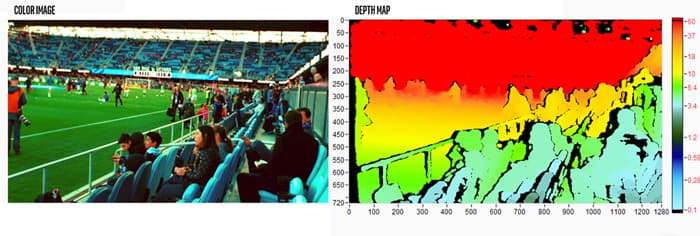
\includegraphics[width=10cm]{./Graphics/rgbd.png}
	\caption{Imagen de color e imagen de profundidad. El color cyan en el mapa de profundidad corresponde a las distancias más cercanas. Tomado de \cite{intel}.}
	\label{fig:rgbd}
\end{figure}

\subsubsection{Tipos de cámaras}

Existe una gran variedad de métodos para calcular profundidad utilizando sensores, cada uno de ellos con sus fortalezas, debilidades y condiciones ideales de operación. A continuación se exponen algunos:

\begin{itemize}
	\item \textbf{Luz estructurada y codificada:} Las cámaras de profundidad que utilizan esta tecnología proyectan una luz (generalmente infrarroja) desde un emisor hacia la escena. La luz proyectada es un patrón visual, un patrón de tiempo o una combinación de estos. El sensor en la cámara detecta el patrón proyectado en la escena y recibe información de profundidad producto de la deformación del mismo. 
	
	Por ejemplo, si el patrón consiste en una serie de líneas que se proyectan sobre una pelota, entonces las líneas deben deformarse alrededor de la superficie de la pelota de una forma específica. Si la pelota se acerca al emisor, el patrón cambia de igual forma. Utilizando la diferencia entre la imagen esperada y la imagen captada por la cámara se puede calcular la distancia hasta la cámara en cada píxel.
	
	\item \textbf{Profundidad estéreo:} Estas herramientas tienen dos sensores colocados a una distancia fija denominada \textit{baseline}. La cámara toma dos imágenes desde los sensores y las compara. Dado que el \textit{baseline} es un valor fijo y conocido, esta comparación entre las imágenes aporta información de profundidad. Estos dispositivos funcionan similar al cerebro y los ojos. Objetos cercanos se mueven significativamente de un ojo a otro, mientras que objetos lejos se mueven muy poco. Las cámaras de profundidad estéreo a menudo proyectan luces infrarrojas hacia la escena para mejorar la precisión de los datos. Las cámaras estéreo utilizan cualquier luz para medir profundidad. Este sistema es el que emplean las cámaras Intel\textregistered~RealSense\texttrademark~Depth Camera D435i.
	
	\item \textbf{Tiempo de vuelo y LiDAR} Toda la tecnología anteriormente descrita se apoya en información conocida para calcular profundidad. Los sensores LiDAR son un tipo de cámaras que utilizan luz láser para calcular profundidad. Emiten una luz sobre la escena y calculan cuanto demora la luz en volver al sensor de la cámara. La confiabilidad de la medición de estas cámaras en distancias significativas depende del poder y longitud de onda de la luz láser.
\end{itemize}

\subsection{Matriz intrínseca de la cámara}\label{section:calibration}

El trabajo teórico con estos dispositivos requiere del diseño de modelos que representen y simulen su comportamiento real. Por este motivo, la literatura abarca diversos esquemas de complejidad variable que describen los distintos tipos de cámaras existentes. Este proyecto se centra en una generalización del modelo de cámara estenopeica o \textit{pinhole camera} que elimina las restricciones sobre los parámetros, conocida como modelo de proyección general.

\begin{definition}
	La matriz del modelo de cámara de proyección general $P$ transforma puntos $\hat{X} = [X, Y, Z]^T$ del mundo real a puntos $\hat{x} = [x, y]^T$ de la imagen según $\hat{X} = P\hat{x}$, siendo $\bar{X} = [X, Y, Z, 1]^T$ el vector extendido de $\hat{X}$ y $\bar{x} = [x, y, 1]^T$ el vector extendido de $\hat{x}$. La matriz P es de dimensión $3 \times 4$ de rango 3, conocida como matriz de la cámara o de proyección y puede factorizarse de la forma \cite{hartley2004camera}:
	\begin{equation}\label{eq:proyGeneral-1}
		P = KR[I| - C] = K[R|t]
	\end{equation}
	\begin{equation}\label{eq:proyGeneral-2}
		t = -RC
	\end{equation}
	Por tanto,
	\begin{equation}\label{eq:proyGeneral-3}
		\begin{pmatrix}
			x\\
			y\\
			1
		\end{pmatrix} = K[R|t] \begin{pmatrix}
			X\\
			Y\\
			Z\\
			1	
		\end{pmatrix}
	\end{equation}
\end{definition}

\begin{figure}[ht]
	\centering
	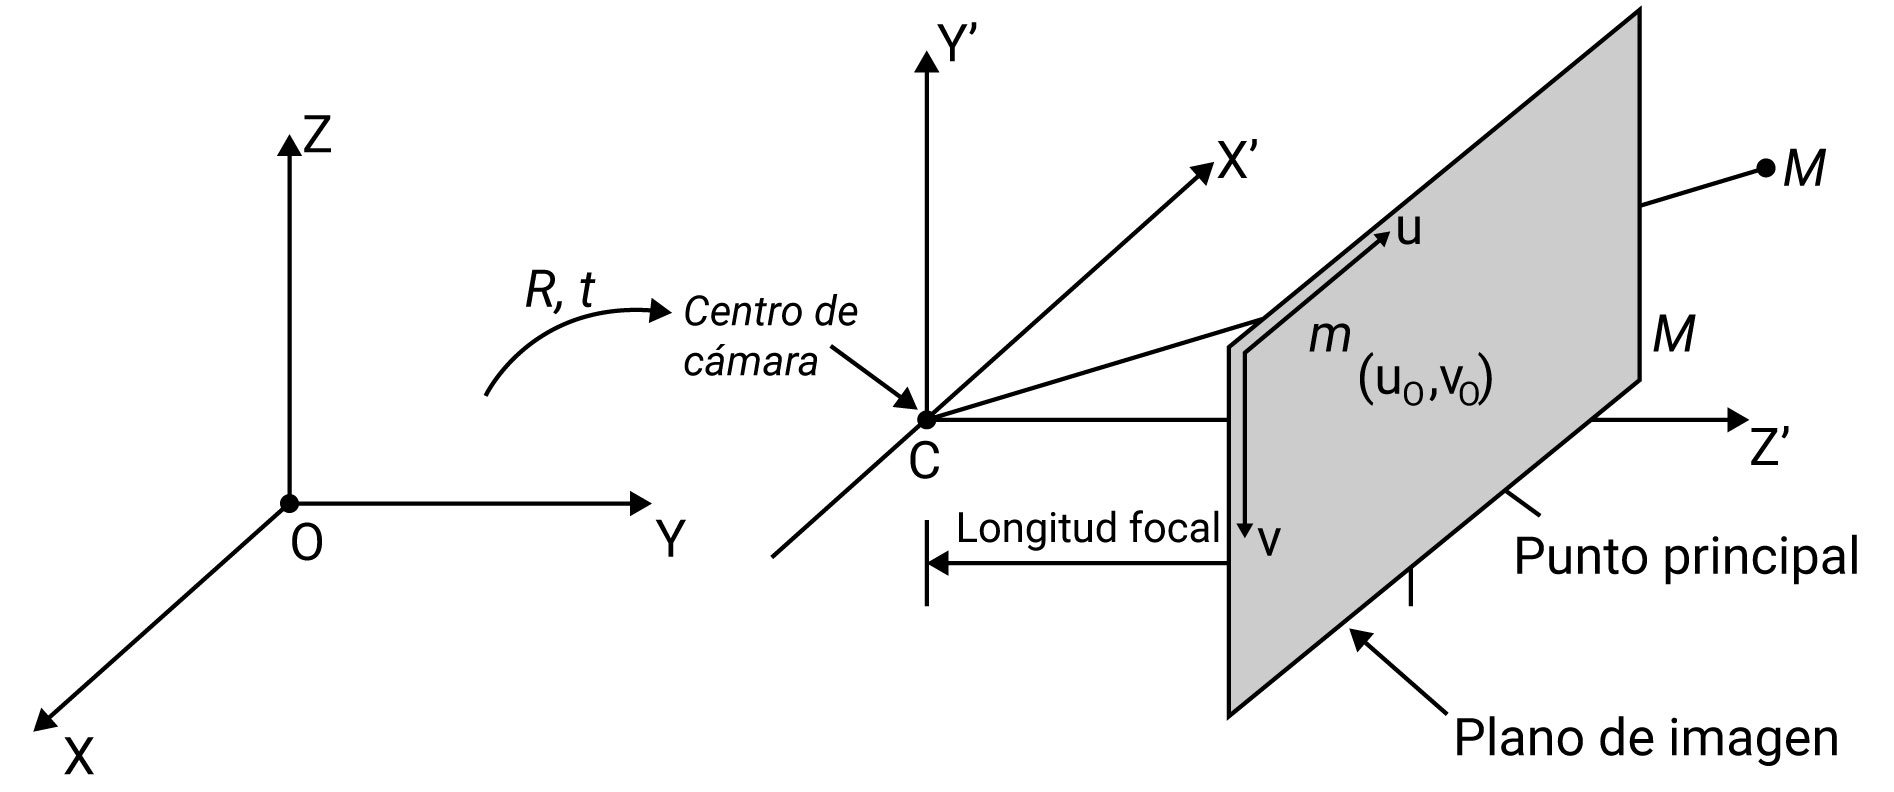
\includegraphics[width=10cm]{./Graphics/modelo-proyeccion-general.png}
	\caption{Modelo de cámara de proyección general. Sistema de coordendas de (a) Objeto o realidad (X, Y, Z), (b) Cámara (X', Y', Z') e (c) Imagen (u, v). Tomada de~\cite{ji2022vision}.}
	\label{fig:proyGeneral}
\end{figure}

En la definición anterior $C$ representa las coordenadas del centro de cámara en el sistema de coordenadas reales (Figura \ref{fig:proyGeneral}(a)) y $R$ es la matriz de rotación de dimensiones $3 \times 3$, que representa la orientación del sistema de coordenadas de la cámara (Figura \ref{fig:proyGeneral} (b)). Los parámetros de $R$ y $C$ son conocidos como externos o de orientación exterior. La notación $[I| - C]$ representa la matriz compuesta por la identidad $I$ junto al vector columna $-C$ y análogamente sucede con $[R|t]$.

La matriz $K$ es conocida como matriz intrínseca o de calibración, la cual es invariante para una misma cámara. Es la encargada de determinar la proyección del sistema de coordenadas de la cámara a coordenadas de la imagen (Figura \ref{fig:proyGeneral} (c)). Como bien su nombre indica está formada por los parámetros internos (intrínsecos) y posee la siguiente estructura:

\begin{equation}
	K = \begin{pmatrix}
		m_x && 0 && 0 \\
		0 && m_y && 0 \\
		0 && 0 && 0 \\
	\end{pmatrix}
	\begin{pmatrix}
		f && \frac{s}{m_x} && p_x \\
		0 && f && p_y \\
		0 && 0 && 1 \\
	\end{pmatrix} =
	\begin{pmatrix}
		a_x && s && x_0 \\
		0 && a_y && y_0 \\
		0 && 0 && 1 \\
	\end{pmatrix}
\end{equation}

donde, $m_x$ y $m_y$ son el número de píxeles por unidades de las coordenadas $x$ y $y$ de la imagen. Por tanto $a_x = fm_x$ y $a_y = fm_y$ constituyen la distancia focal $f$ representada en número de píxeles respecto a las direcciones $x$ y $y$. De igual manera ($x_0 = p_xm_x, y_0 = p_ym_y$) son las coordenadas del punto principal $(p_x, p_y)$ en términos de número de píxeles. El valor de $s$ (skew), indica la desviación de rectangularidad. Sin embargo, para cámaras usuales se asume $s=0$.

Tanto los parámetro internos como los externos son adquiridos a partir de la calibración geométrica del sistema.

\begin{definition}
	La calibración geométrica es el proceso de determinación de las propiedades geométricas de la cámara. Su propósito es descubrir la correspondencia entre rayos y puntos de la imagen \cite{kannala2008geometric}.
\end{definition}

El método de calibración que se detalla a continuación, es el usado en las cámaras Intel\textregistered~RealSense\texttrademark~de la serie D400 y detallado en \cite{grunnet2021intel}, donde se describe un conjunto de componentes integrados en el \textit{Software Develpment Kit} (SDK 2.0) de Intel\textregistered~RealSense\texttrademark~llamado \textit{Self-Calibration} o Auto-Calibración. 

\subsection{Método de calibración}

EL conjunto de componentes integrados conocido como Auto-Calibración se emplea con el objetivo de (1) restaurar el rendimiento de la profundidad y (2) mejorar la exactitud de un dispositivo Intel\textregistered~RealSense\texttrademark~Depth Camera D400 que pueda verse degradado con el tiempo. A diferencia de otros procedimientos, este no requiere movimiento ni reposicionamiento durante la calibración y puede completarse en cuestión de segundos. El método propuesto en \cite{grunnet2021intel} es rápido y no sobrecarga la Unidad Central de Procesamiento (CPU).

A continuación se describen uno de los métodos de auto-calibración, se expresan sus beneficios, restricciones e instrucciones.

\subsubsection{Calibración de la cámara minimizando el ruido en la profundidad}

El método que se explica calibra la cámara buscando optimizar el rendimiento de la medición de profundidad en términos de minimizar el ruido en la misma con el sistema estéreo. Se enfoca en la habilidad de los dispositivos de observar un objeto y reportar la posición de estos con bajo nivel de ruido, en otras palabras, se refiere al mejoramiento de la precisión o el error relativo de la medición.

Para visualizar los niveles de ruido en profundidad en las cámaras se recomienda apuntar hacia una pared plana. Las cámaras de la serie D400 bajan su rendimiento de acuerdo a la distancia al objeto gradualmente mostrando cada vez más ruido en el mapa de profundidad. Por esta razón, al apuntar hacia la pared se muestran cada vez más variaciones en la medición de profundidad y se obtienen con más frecuencia valores 0 indicando profundidades inválidas (Figura \ref{fig:calibration}). Para cuantificar la precisión en la profundidad o el error relativo, las cámaras se apuntan a la pared plana u otro objetivo plano y se mide la profundidad en cada punto de la pequeña sección conocida como Campo de visión o FOV por sus siglas en inglés \textit{field-of-view}, que por lo general es el 10\% o 20\% de la región de interés cerca del centro. Como se asume que el objetivo es plano, entonces, el mapa de profundidad de la región de interés se ajusta a un plano y el error cuadrático medio (RMS por sus siglas en inglés) se mide como la desviación estándar del plano.

\begin{figure}[ht]
	\centering
	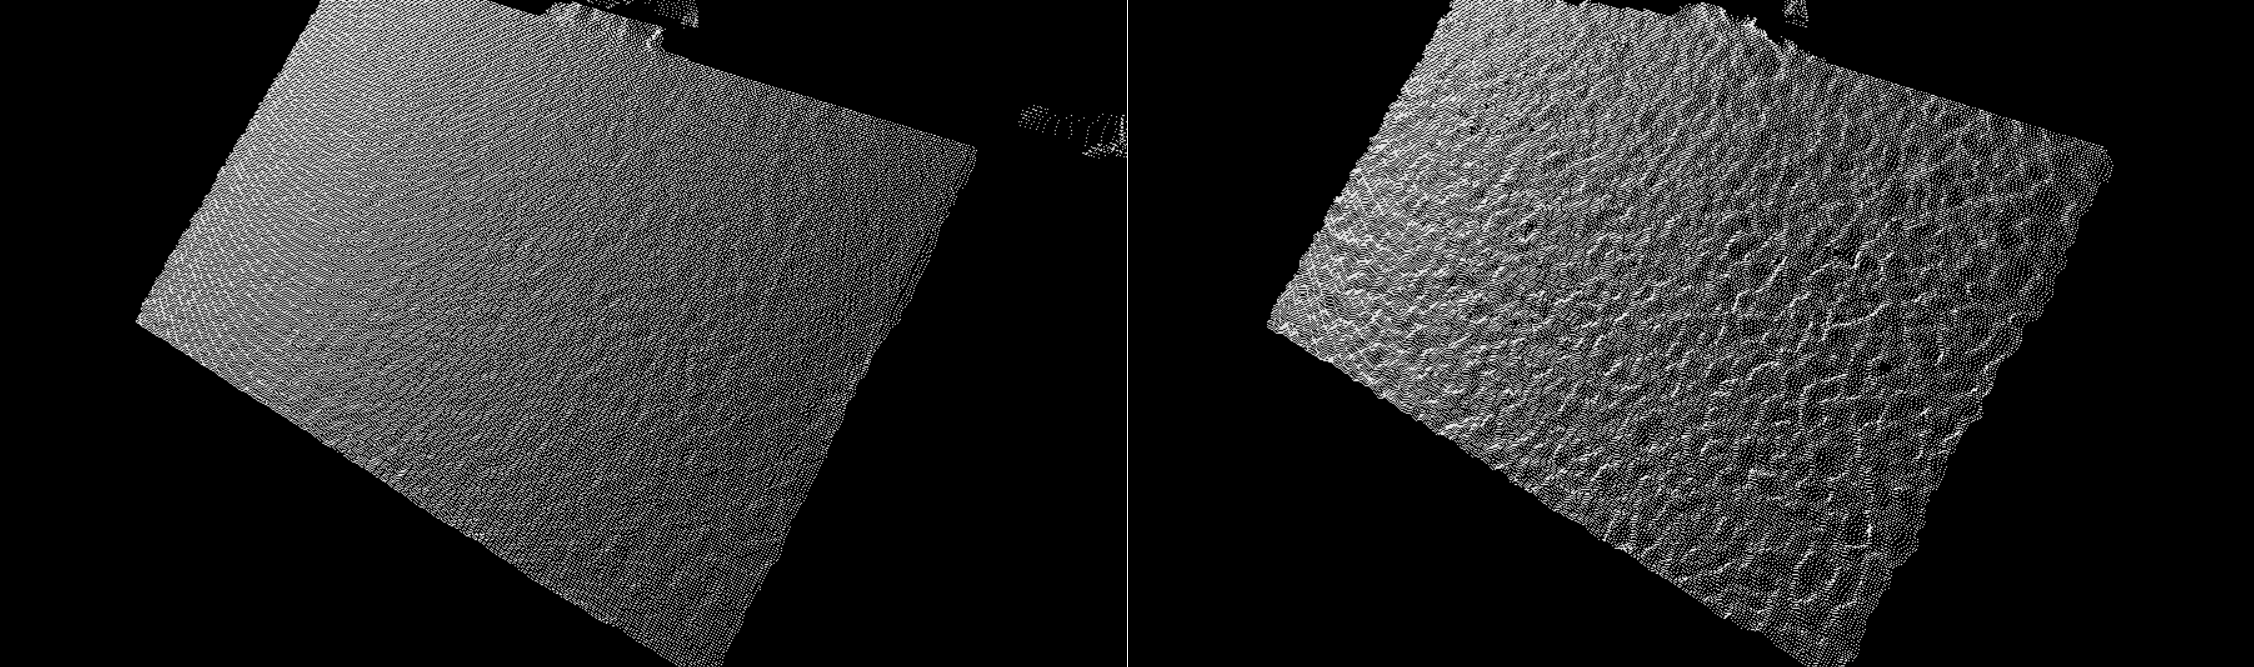
\includegraphics[width=10cm]{./Graphics/calibration.png}
	\caption{Comparación de las nubes de puntos obtenidas de una cámara bien calibrada (izquierda) y una cámara descalibrada (derecha). Ambas apuntando hacia la pared plana.}
	\label{fig:calibration}
\end{figure}

El rendimiento puede ser reportado en unidades absolutas como milímetros o centímetros, pero la forma de comparar y reportar el rendimiento entre cámaras, rangos de profundidad, resoluciones, FOV y variaciones del proyector es utilizar una métrica normalizada llamada \textit{Subpixel RMS} ($\sigma_{RMS}$) \cite{grunnet2021intel}:

\begin{equation}
	\sigma_{RMS}(px) = \frac{\phi(px) * \beta(m) * \epsilon_{DepthRMS}(mm)}{\delta(mm)^2}
\end{equation}

donde:

\begin{itemize}
	\item $\phi$ es la distancia focal del sensor de profundidad, se cumple que $\phi = \frac{Xres(px)}{2\tan(\frac{HFOV}{2})}$.
	\item $\epsilon_{DepthRMS}$ es el ruido del plano ajustado.
	\item $\beta$ es el \textit{baseline} o distancia entre los sensores de la cámara RGB.
	\item $\delta$ es la distancia desde la cámara hacia la pared plana u objetivo plano.
	\item \textit{HFOV} es el campo de visión horizontal de los sensores estéreo.
	\item \textit{Xres} es la resolución horizontal del mapa de profundidad sobre la que se hace la medición de la profundidad, por ejemplo 1280 o 848 píxeles.
\end{itemize} 

Los parámetros \textit{HFOV}, $\beta$, $\phi$ y \textit{Xres} se obtienen de la matriz intrínseca de la cámara. 

\subsubsection{Optimización de la exactitud de la medición de profundidad}

El método que se describe a continuación para la optimización de la exactitud de la medición de profundidad hace referencia al mejoramiento de la medición de distancia hacia el valor más preciso posible.

El algoritmo recibe como entrada la distancia exacta que debe medir en el plano perpendicular desde el sensor RGB izquierdo, esta distancia se denomina \textit{ground truth}. Es todo un desafío obtener un \textit{ground truth} de calidad. Se debe asegurar antes de ejecutar el algoritmo que el objetivo sea plano y perpendicular al eje óptico de la cámara, además, el mapa de profundidad debe ser bueno (esto es, haber ejecutado el método descrito anteriormente). La ejecución de este algoritmo es rápida con un tiempo de ejecución entre 30ms y 1 segundo. 

Este método realiza pequeños ajustes a la matriz intrínseca de la cámara para producir un mapa de profundidad que en promedio sean cercanos al \textit{ground truth}. 

\section{Técnicas de pre/postprocesamiento en el mejoramiento de imágenes}\label{section:imgEnh}

Una de las principales tareas en el procesamiento de imágenes digitales es el mejoramiento de estas con el fin ajustarlas para su visualización o proveerlas como entrada a algoritmos. Entre las técnicas de mejoramiento de imágenes se encuentra la eliminación de ruido, el mejoramiento de contraste, la aplicación de filtros y operadores morfológicos y la manipulación del histograma.

Para las explicaciones teóricas de la presente sección se consideran las imágenes en escala de grises ($k=1$ en \ref{def:img}). Todas las operaciones y explicaciones pueden ser extendidas a imágenes RGB aplicándolas en cada canal de color.

\subsection{Mejoramiento de contraste: CLAHE}

A menudo, los objetos presentes en las imágenes no se diferencian entre ellos, producto del bajo contraste en la fotografía. Existen técnicas para ajustar los niveles de contraste en una imagen.

\begin{definition}
	El histograma de una imagen $I_{n \times m}$ se define como la función de distribución de los niveles de intensidad de la imagen.
\end{definition}

\begin{definition}
	Se define como contraste en una imagen la diferencia de intensidad de gris de los píxeles presentes en la imagen.
\end{definition}

La ecualización del histograma es una de las técnicas que permiten el ajuste del contraste. La ecualización se concibe como una transformación o manipulación de la imagen con el fin de obtener un histograma con distribución uniforme de valores de intensidad. En teoría, la aplicación de esta operación debería transformar el histograma en otro con una forma perfectamente uniforme sobre todos los niveles de gris. Sin embargo, en la práctica esto no se va a poder conseguir pues se estaría trabajando con funciones de distribución discretas en lugar de continuas. En la transformación, todos los píxeles de un mismo nivel de gris se transformarán a otro nivel de gris y el histograma se distribuirá en todo el rango disponible separando en lo posible las ocupaciones de cada nivel. El resultado de la ecualización maximiza el contraste de una imagen sin perder información de tipo estructural \cite{solomon2011fundamentals}, esto es, conservando su entropía~\footnote{La entropía es una medida de la información contenida en una imagen y los estados de niveles de intensidad de los píxeles.}.

\subsubsection{CLAHE}

La ecualización del histograma produce buenos resultados en el mejoramiento de las imágenes. La ecualización adaptativa del histograma (AHE, por sus siglas en inglés) calcula varios histogramas, cada uno de ellos correspondiente a una sección distinta de la imagen y los utiliza para redistribuir los valores de luminosidad de la imagen.  Sin embargo, AHE amplifica demasiado el ruido en regiones relativamente homogéneas de una imagen. El algoritmo de Ecualización Adaptativa del Histograma con Limitación de Contraste (CLAHE, por sus siglas en inglés) pretende aportar una solución al problema anterior. 

CLAHE es una variante de ecualización adaptativa del histograma en la que la amplificación de contraste es limitada. La amplificación del contraste en las proximidades de un valor de píxel, viene dada por la pendiente de la función de transformación. Esto es proporcional a la pendiente de la función de distribución acumulativa de vecindad (CDF) y, por lo tanto, al valor del histograma en ese valor de píxel.  CLAHE limita la amplificación recortando el histograma a un valor predefinido antes de calcular el CDF. Esto limita la pendiente de la CDF y, por tanto, de la función de transformación. El valor al que se recorta el histograma, el llamado límite de recorte, depende de la normalización del histograma y, por tanto, del tamaño de la región de vecindad~\cite{pizer1987adaptive}. Los valores comunes limitan la amplificación resultante entre 3 y 4.
 
Es ventajoso no descartar la parte del histograma que excede el límite de recorte, sino redistribuirlo por igual entre todos los contenedores de histogramas.


\subsection{Filtros}

Los filtros digitales constituyen uno de los principales modos de operar en el procesamiento de imágenes digitales. Los filtros suelen usarse para distintos fines como el suavizado, acentuado de imágenes, eliminación de ruido y detección de bordes, pero en todos los casos, el resultado sobre cada píxel depende de los píxeles de su entorno. Una imagen se puede filtrar en el dominio del espacio, trabajando directamente sobre los píxeles de la imagen, o en el dominio de la frecuencia, donde las operaciones se llevan a cabo en la transformada de Fourier de la imagen.

Los filtros lineales en particular, se basan en máscaras de convolución~\footnote{Una máscara de convolución no es más que una matriz de coeficientes.}. Dada una imagen $I_{h \times w}$ y una máscara de convolución $M$ la imagen resultante $G_{h \times w}$ consiste en realizar la operación de convolución $W * I$.

\begin{definition}
	Dado el filtro $W[x, y]$ de tamaño $m \times n$ y la imagen $I_{h \times w}$, la convolución entre $W$ e $I$, denotada como $W * I$ está dada por la ecuacion:
	
	\begin{equation}
		W * I = \sum_{s = -a}^a\sum_{t = -b}^b W[s,t] I[x - s, y - t]
	\end{equation}

	Con $a = \frac{m -1}{2}$ y $b = \frac{n -1}{2}$. Se asume por conveniencia de notación que $n, m \in \mathbb{Z}$ y $n, m$ son impares.
\end{definition}



\subsubsection{Filtro Gaussiano}

El filtro gaussiano se usa para emborronar imágenes y eliminar el ruido de Gauss, pues preserva los bordes a medida que suaviza la imagen reduciendo los niveles de ruido. El mismo se define como aquel cuya respuesta al impulso es una función gaussiana o una aproximación a ellas.

\begin{equation}
	\frac{1}{2\pi\sigma^2} e^{-\frac{x^2 + y^2}{2\sigma^2}}
\end{equation}

\subsubsection{Filtro de Acentuado o \textit{Sharpening}}

El filtro \textit{sharpening} se utiliza para acentuar y definir los bordes la imagen. La máscara de convolución empleada es la siguiente:

\begin{equation}
	M = \begin{pmatrix} 
		0 & -1 & 0 \\
		-1 & 5 & -1 \\ 
		0 & -1 & 0
	\end{pmatrix}
\end{equation}

La máscara de convolución anterior se obtiene de aplicar el filtro de Laplace de detección de bordes y adicionarle la imagen original a la imagen resultante del filtrado laplaciano~\cite{sharpen}.

\subsection{Filtros de imágenes de profundidad}

Para obtener la mejor calidad en los mapas de profundidad en ocasiones es necesaria la aplicación de filtros. El SDK de Intel\textregistered~RealSense\texttrademark incluye filtros de postprocesamiento para mejorar la calidad de los datos de profundidad y reducir los niveles de ruido. Todos los filtros se implementan en el núcleo de la biblioteca.

Para la mayoría de los casos de uso no es necesaria una gran cantidad de puntos, esto también puede perjudicar el rendimiento a la hora de aplicar filtros más potentes. Por esta razón se considera primeramente realizar un filtro de Decimación, así se reduce la resolución espacial preservando la $z$-exactitud.

\subsubsection{Filtro de decimación}

En lugar de reducir el tamaño de la nube de puntos tomando un píxel por cada $n$, se realiza un submuestreo más inteligente. El filtro se ejecuta en tamaños de \textit{kernel} $2 \times 2$ a $8 \times 8$ píxeles. Para bloques de tamaño 2 y 3, se selecciona el valor de profundidad  de \textquotedblleft mediana sin ceros\textquotedblright . Para dimensiones de \textit{kernel} más grandes, de 4 a 8 píxeles, se utiliza el valor de la \textquotedblleft media sin ceros\textquotedblright . Si bien esto afectará claramente la resolución $x-y$ del mapa de profundidad, se debe tener en cuenta que los algoritmos de visión estereoscópica involucran algunas operaciones de convolución, por lo que reducir la resolución $x-y$ después de la captura con un submuestreo modesto conducirá a un impacto bastante mínimo en la resolución $x-y$ de profundidad. 

Uno de los beneficios del submuestreo inteligente es que también hará un poco de relleno rudimentario y suavizará los datos . El \textquotedblleft sin ceros\textquotedblright\ se refiere al hecho de que los valores en el mapa de profundidad que son cero deben ignorarse. Estos son \textquotedblleft agujeros\textquotedblright\ en el mapa que representan datos de profundidad que no cumplieron con la métrica de confianza y en lugar de proporcionar un valor incorrecto, la cámara proporciona un valor de cero en ese punto. Una vez comprimido el mapa de profundidad, se pueden aplicar filtros espaciales y temporales.

\subsubsection{Filtro espacial con conservación de aristas}

Su implementación se describe en~\cite{gastal2011domain}. Este tipo de filtros suaviza el ruido mientras intenta conservar las aristas. Considere el ejemplo de la figura \ref{fig:space1}, las mediciones ideales serian las presentadas en la parte izquierda. Al aplicar varios filtros para suavizar, se puede notar que el ruido disminuye, pero también se suavizan las aristas como se muestra en la figura \ref{fig:space2}.

\begin{figure}[ht]
	\centering
	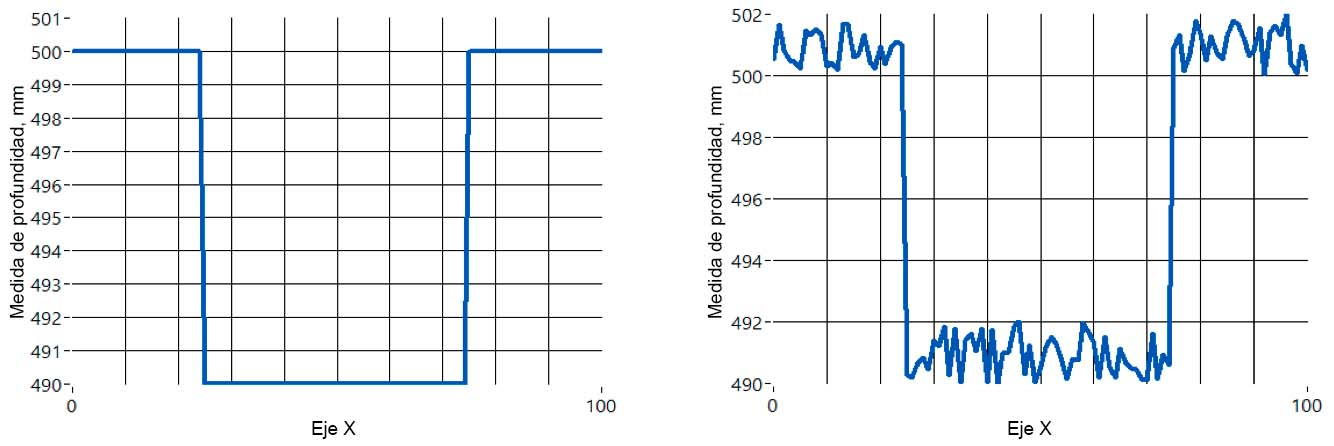
\includegraphics[width=10cm]{./Graphics/figura1.png}
	\caption{Comparación de las mediciones de profundidad. (Izquierda) medición ideal, (Derecha) medición con ruido}
	\label{fig:space1}
\end{figure}

\begin{figure}[ht]
	\centering
	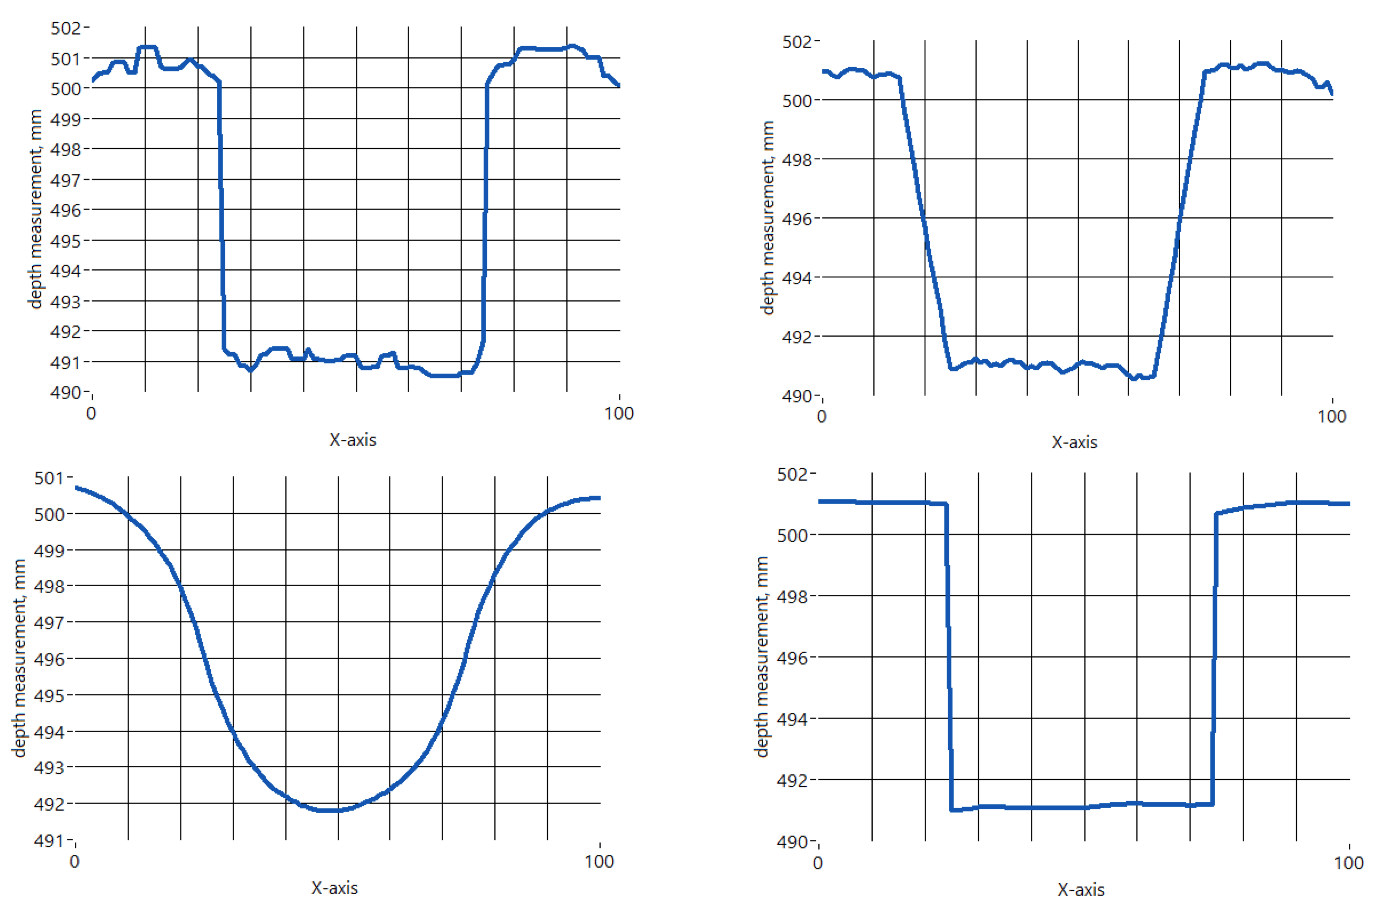
\includegraphics[width=10cm]{./Graphics/figura2.png}
	\caption{En la parte superior izquerda se realiza un filtro promedio, en la parte	superior derecha se aplica EMA unidireccional, en la parte inferior izquerda se aplica EMA bidireccional y en la parte inferior derecha el filtro propuesto.}
	\label{fig:space2}
\end{figure}

Para este filtro, se escanea el mapa de profundidad en el eje $X$ y el eje $Y$ y viceversa, dos veces, mientras se calcula el Promedio Móvil Exponencial (EMA, por sus siglas en inglés) unidimensional usando un parámetro $\alpha$ que determina la cantidad de suavizado. La ecuación recursiva específica es:

\begin{equation}
	S_t = \left\{ \begin{array}{lcc}
		Y_1 & &  t = 1\\
		\\ \alpha Y_t + (1-\alpha)S_{t-1} &  &t > 1 \wedge \Delta=|S_t - S_{t-1} < \delta_{thresh}|\\
		\\ Y_t & & t > 1 \wedge \Delta=|S_t - S_{t-1} > \delta_{thresh}|
	\end{array}
	\right.
\end{equation}

El coeficiente $\alpha$ representa el grado de disminución de la ponderación. $Y_t$ es el valor recién registrado (de disparidad o profundidad) y $S_{t-1}$ es el valor de la EMA en el tiempo $t$. También se agrega un parámetro de umbral denotado $\delta_{thresh}$. Si el valor de profundidad entre los píxeles vecinos excede el umbral de profundidad establecido por este parámetro $\delta_{thresh}$, entonces $\alpha$ se restablecerá temporalmente a 1 (sin filtrado). Básicamente, esto significa que si se observa un borde, el suavizado se desactiva temporalmente.


\subsubsection{Filtro de relleno de agujeros}

Para lidiar con los \textquotedblleft agujeros\textquotedblright\ que pueden ocurrir debido a oclusión o falta de textura en la superficie se utiliza un método simple. El filtro obtiene los cuatro píxeles vecinos inmediatos (arriba, abajo, izquierda, derecha) y selecciona uno de ellos de acuerdo con una regla predefinida.

\subsubsection{Filtro temporal}

Siempre que sea posible, es recomendado tener en cuenta los \textit{frames} anteriores para promediar los mapas de profundidad, sobre todo para escenas de naturaleza estática. Los cambios de luz, o movimientos inherentes al sensor, pueden introducir ruido en los mapas de profundidad. Para reducir este ruido se aplica el mismo filtro espacial descrito anteriormente, solo que ahora entre \textit{frames}. Al configurar $\alpha = 1$, habrá cero filtrado, pero acercar $\alpha$ a 0 aumentará el promedio y la suavidad. Por lo tanto, no es un simple ``promedio de 2, 3 o 4 frames'', sino que permite un suavizado mas refinado. Además, al igual que con el filtro espacial, es importante agregar un parámetro de umbral. De esta manera se trata de reducir el suavizado temporal cerca de los bordes y tampoco se incluyen agujeros ($z=0$) en el promedio.

\subsection{Morfología matemática}

La palabra morfología se refiere a la forma y estructura de algún elemento, en el campo del procesamiento de imágenes se utiliza para referirse a la forma de una región en la imagen. La morfología matemática es una metodología basada en la teoría de conjuntos y la topología, que intenta de una manera cuantitativa describir la estructura de objetos en una imagen~\cite{bovik2009essential}.

Las operaciones morfológicas fueron originalmente definidas como operaciones sobre conjuntos y han demostrado ser útiles para procesar puntos en un espacio de dos dimensiones. Estas utilizan una estructura conocida como elemento estructurante~\cite{soille1999morphological, haralick1987image}.

\begin{definition}
	Se define una imagen binaria $B_{h \times w}$ como una imagen, tal que: $B_{h \times w}[i, j] = p_{i, j} \in \{0, 1\}$ y $0 \leq i \leq h - 1$, $ 0 \leq j \leq w-1$.
\end{definition}

\begin{definition}
	Se define un elemento estructurante $S$ como una imagen binaria $S_{a \times b}$ representando un tamaño y forma arbitrarios.
\end{definition}

Los elementos estructurantes se utilizan para hacer un proceso similar a la convolución aplicando una operación lógica entre el elemento estructurante $S$ y cada píxel $p_{i, j} \in B_{h \times w}$. El resultado de esta operación se almacena en cada píxel. El efecto que se obtiene depende del tamaño y la forma del elemento estructurante $S$~\cite{castleman1996digital} (Figuras \ref{fig:estructurante} y \ref{fig:kernel}).

\begin{figure}[ht]
	\centering
	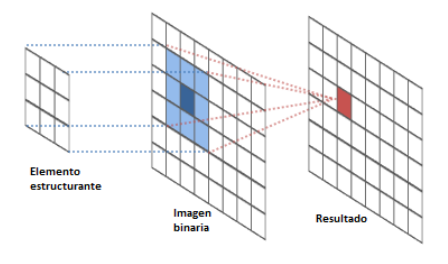
\includegraphics[width=10cm]{./Graphics/estructurante.png}
	\caption{Representación de una operación morfológica con un elemento estructurante}
	\label{fig:estructurante}
\end{figure}	

\begin{figure}[ht]
	\centering
	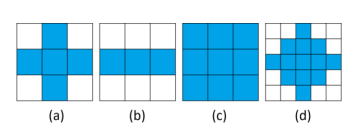
\includegraphics[width=10cm]{./Graphics/kernel.png}
	\caption{Elementos estructurales. (a) cruz, (b) línea, (c) rectángulo de 3$\times$3 y en (d) el disco de radio 2.}
	\label{fig:kernel}
\end{figure}

\subsubsection{Operaciones básicas}

Existen dos operaciones morfológicas básicas  muy empleadas en el procesamiento de imágenes. Antes de presentarlas se definen algunos conceptos importantes para la comprensión de las mismas.

\begin{definition}
	Dos píxeles $P_t$ y $P_k$ están conectados si son adyacentes en la imagen en cualquiera de las ocho direcciones.
\end{definition}

\begin{definition}
	Un camino entre un par de píxeles $P_t$ y $P_k$ es una secuencia $P_t = P_1, P_2, \ldots,$ $P_e = P_k$ tal que $P_i$ y $P_{i + 1}$ están conectados $\forall 1 \leq i \leq e$.
\end{definition}

\begin{definition}
	Una región es un conjunto de píxeles conectados de tal forma que entre todo par de píxeles existe un camino.
\end{definition}

\begin{definition}
	Un punto frontera $P_{i, j}$ es un píxel que pertenece a una región pero que al menos uno de sus vecinos no lo está.
\end{definition}

\begin{itemize}
	\item \textbf{Erosión:} La erosión es el proceso de eliminar todos los puntos fronteras de una región, convirtiendo el objeto más pequeño en área por un píxel sobre todo su perímetro. La erosión es útil para remover objetos de una imagen segmentada que pueden ser muy pequeños para ser de interés~\cite{castleman1996digital}. En general, se puede definir de la siguiente manera:
	
	\begin{equation}
		E = B \otimes S = \{x, y | S_{x, y} \subseteq B\}
	\end{equation}

	\item \textbf{Dilatación:} La dilatación es el proceso de incorporar a una región todos los puntos fuera de la misma que sean adyacentes a esta, dejándola más grande en área por esa cantidad de puntos. La dilatación se puede utilizar para rellenar huecos en regiones segmentadas~\cite{castleman1996digital}. En general, se puede definir de la siguiente manera:
	
	\begin{equation}
		D = B \otimes S = \{x, y | S_{x, y} \cap B \neq \emptyset\}
	\end{equation}
\end{itemize}

Con estas operaciones combinadas se puede realizar la operación conocida como cerrado.

\subsubsection{Cerrado}

Este proceso consiste en aplicar el operador básico dilatación y al resultado aplicarle el operador erosión. Tiene el efecto de llenar pequeños huecos en las regiones, conectar objetos cercanos y generalmente, suavizar la frontera de un objeto sin cambio significativo en su área~\cite{castleman1996digital}. Se define el proceso de la siguiente manera:

\begin{equation}
	B \bullet S = (B \otimes S) \otimes S
\end{equation}

\section{Seguimiento de objetos visuales a corto plazo}\label{section:tracking}

El Seguimiento de objetos visuales a corto plazo o \textit{Short-term visual object tracking} es el problema en visión computacional que busca localizar continuamente un objetivo en una secuencia de vídeo dada una sola vista del objeto. La comunidad ha prestado una atención importante publicando numerosos artículos proponiendo diversos algoritmos y métricas de evaluación. El problema es desafiante producto de diversos factores como puede ser la oclusión, cambios de iluminación, movimientos bruscos del objeto o la cámara, deformaciones rígidas o no de la apariencia, así como el parecido del fondo con el objeto.	

El algoritmo utilizado para el seguimiento de la úlcera en la secuencia de vídeo es CSR-DCF por sus siglas en inglés \textit{Discriminative Correlation Filter with Channel and Spatial Reliability} propuesto en~\cite{lunevzivc2018discriminative}. La implementación utilizada es la propuesta por la biblioteca \textit{OpenCV}~\cite{bradski2000opencv}.

\subsection{CSR-DCF}\label{sec:csr}

La idea básica tras los algoritmos de seguimiento basados en filtros de correlación es estimar el filtro a través del cual se produce una respuesta deseada a partir de una imagen de entrada. La respuesta deseada es de una forma gaussiana centrada en la ubicación del objeto a seguir.

El filtro se entrena a partir de instancias traducidas del parche objetivo. Al probar, se evalúa la respuesta del filtro y el máximo da la nueva posición del objeto. El filtro se entrena en tiempo real y se actualiza sucesivamente con cada cuadro para que el rastreador se adapte a cambios moderados del objeto.

La principal ventaja de los algoritmos de filtros de correlación es la eficiencia computacional. La razón es que el cálculo se puede realizar en el dominio de Fourier de forma eficiente~\cite{henriques2014high}. 

Este algoritmo utiliza mapas de confiabilidad espacial para ajustar el soporte del filtro a la parte de la región seleccionada del cuadro para el seguimiento, lo que brinda la capacidad de aumentar el área de búsqueda y rastrear objetos no rectangulares. Los índices de confiabilidad reflejan la calidad de los filtros estudiados por canal y se utilizan como pesos para la localización~\cite{lunevzivc2018discriminative}. Por lo tanto, usando el Histograma de Gradientes Orientados (HoG por sus siglas en inglés) y los canales de color RGB como conjuntos de características, el algoritmo funciona relativamente bien.


\section{Segmentación de imágenes}\label{section:seg}

La segmentación de imágenes es un proceso importante en el procesamiento de imágenes digitales. La segmentación se refiere al proceso de particionar una imagen en un grupo de regiones homogéneas y significativas, de tal manera que todos los píxeles en una región posean un conjunto similar de propiedades y atributos~\cite{sundararajan2017digital}. El resultado de la segmentación es un número de regiones donde a cada uno de sus píxeles le corresponde una etiqueta. De esta forma, se puede definir una imagen segmentada como un conjunto de regiones conectadas y no solapadas, donde cada píxel corresponde a una única etiqueta que indica a qué región pertenece.

Formalmente, se puede definir la segmentación de imágenes de la siguiente manera~\cite{pal1993review}:

\begin{definition}
	Si $P$ es una función de similitud entre grupos de píxeles, entonces la segmentación es una partición del conjunto $F$ en regiones conectadas ($R_1, R_2, \ldots, R_t$) tal que:
		\begin{itemize}
			\item $\cup_{i=1}^t R_i = F$
			\item $R_i \cap R_j = \emptyset$ con $i \neq j$.
			\item $P(R_i)$ es verdadero $\forall R_i \in F$.
			\item $P(R_i \cap R_j)$ es falso para toda región adyacente $P(R_i)$ y $P(R_j)$.
		\end{itemize}
\end{definition}

Las técnicas de segmentación pueden ser categorizadas en dos tipos básicos basados en las propiedades de las imágenes:

\begin{itemize}
	\item \textbf{Basado en la detección de discontinuidad}: Una imagen es segmentada en regiones basado en las diferencias entre las regiones~\cite{sundararajan2017digital}.
	\item \textbf{Basado en la detección de similitud}: Las regiones se forman encontrando partes similares en la imagen basado en un criterio definido~\cite{sundararajan2017digital}.
\end{itemize}

Existen diferentes técnicas de segmentación que subcategorizan estos dos tipos básicos~\cite{anjna2017review}. Uno de ellos es la \textbf{segmentación semántica} que se presentará con más detalle a continuación.

\subsubsection{Segmentación semántica}

La segmentación semántica, es también conocida como clasificación a nivel de píxeles. Consiste en agrupar partes de una imagen que correspondan a una misma clase~\cite{thoma2016survey} con el objetivo de entender qué existe en una imagen a nivel de píxeles (Figura \ref{fig:semseg}).

\begin{figure}[ht]
	\centering
	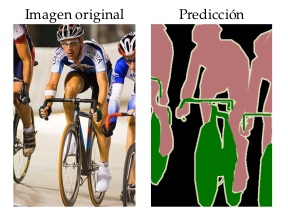
\includegraphics[width=6.5cm]{./Graphics/semseg.png}
	\caption{Resultado de una segmentación basada en píxeles. Cada color en la predicción representa una clase distinta.}
	\label{fig:semseg}
\end{figure}

\begin{property}
	Luego de la clasificación a nivel de píxeles sobre una imagen $I_{h \times w}$ a cada píxel $p_{i, j} \in I_{h \times w}$ le corresponde una única clase $w_k \in W: k \in \mathbb{N}^+$ y $W$ es un conjunto finito de clases predefinidas.
\end{property}

\subsection{Segmentación con redes neuronales}\label{sec:nn}

Según \cite{pham2000survey}, los métodos de segmentación pueden dividirse en 8 categorías:
\begin{enumerate}
\item de aplicación de umbral,
\item de crecimiento de regiones,
\item de clasificación,
\item de agrupamiento,
\item acercamientos por modelos de campos aleatorios de Markov,
\item por modelos deformables,
\item por guía de atlas
\item por redes neuronales artificiales.
\end{enumerate}

Las Redes Neuronales Artificiales (RNA) representan un paradigma en el Aprendizaje de Máquinas y pueden usarse para la segmentación de imágenes de una gran variedad de formas. Las RNA se inspiran en el funcionamiento de las neuronas humanas.

Estructuralmente, una RNA es modelada utilizando capas formadas por neuronas artificiales (unidades computacionales). Las unidades entre capas están conectadas por enlaces. Un enlace de la unidad $i$ a la $j$ sirve para propagar la activación $a_i$. Además, cada conexión tiene asociado un peso $w_{ij}$ que determina la fortaleza de dicho enlace. Cada neurona $j$ calcula una suma ponderada de sus entradas de la forma $in_j = \displaystyle\sum_{i = 0}^{n} w_{ij}a_i$ y luego aplica una función de activación $g$ sobre $in_j$, para obtener su salida $a_j = g(in_j)$. En un modelo simple la primera capa es la llamada entrada, las intermedias se conocen como capas ocultas y por último tenemos la capa de salida. En la Figura \ref{fig:rna} se muestra la estructura básica de una Red Neuronal Artificial simple.

\begin{figure}[ht]
	\centering
	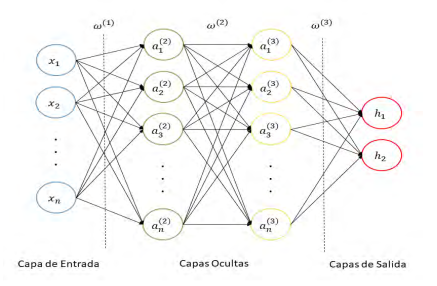
\includegraphics[width=10cm]{./Graphics/rna.png}
	\caption{Ejemplo de una arquitectura de RNA con dos capas ocultas.}
	\label{fig:rna}
\end{figure}

Existe un tipo de RNA conocido como Redes Neuronales Convolucionales (RNC), comúnmente aplicado al análisis de imágenes digitales. Su nombre indica el empleo de la convolución.

En los últimos años, este tipo de arquitectura de RNA ha tomado gran auge dentro de la tarea de segmentación. Las próximas secciones presentan dos Redes Neuronales Convolucionales orientadas a la segmentación de imágenes médicas.

\subsubsection{UNet}

UNet es una arquitectura de RNC orientada a la segmentación. Esta red cuenta con la capacidad de localizar objetos o clases, es decir, a cada píxel le asigna una etiqueta con su clase. Su mayor ventaja es que a diferencia de otras arquitecturas requiere de pocas muestras anotadas para lograr su propósito; pues su estructura y estrategia de entrenamiento, que recae en el aumento de los datos, hacen uso eficiente de las imágenes. Este último rasgo es muy beneficioso en el procesamiento de imágenes médicas, donde adquirir grandes volúmenes de información es una tarea usualmente compleja.

\begin{figure}[ht]
	\centering
	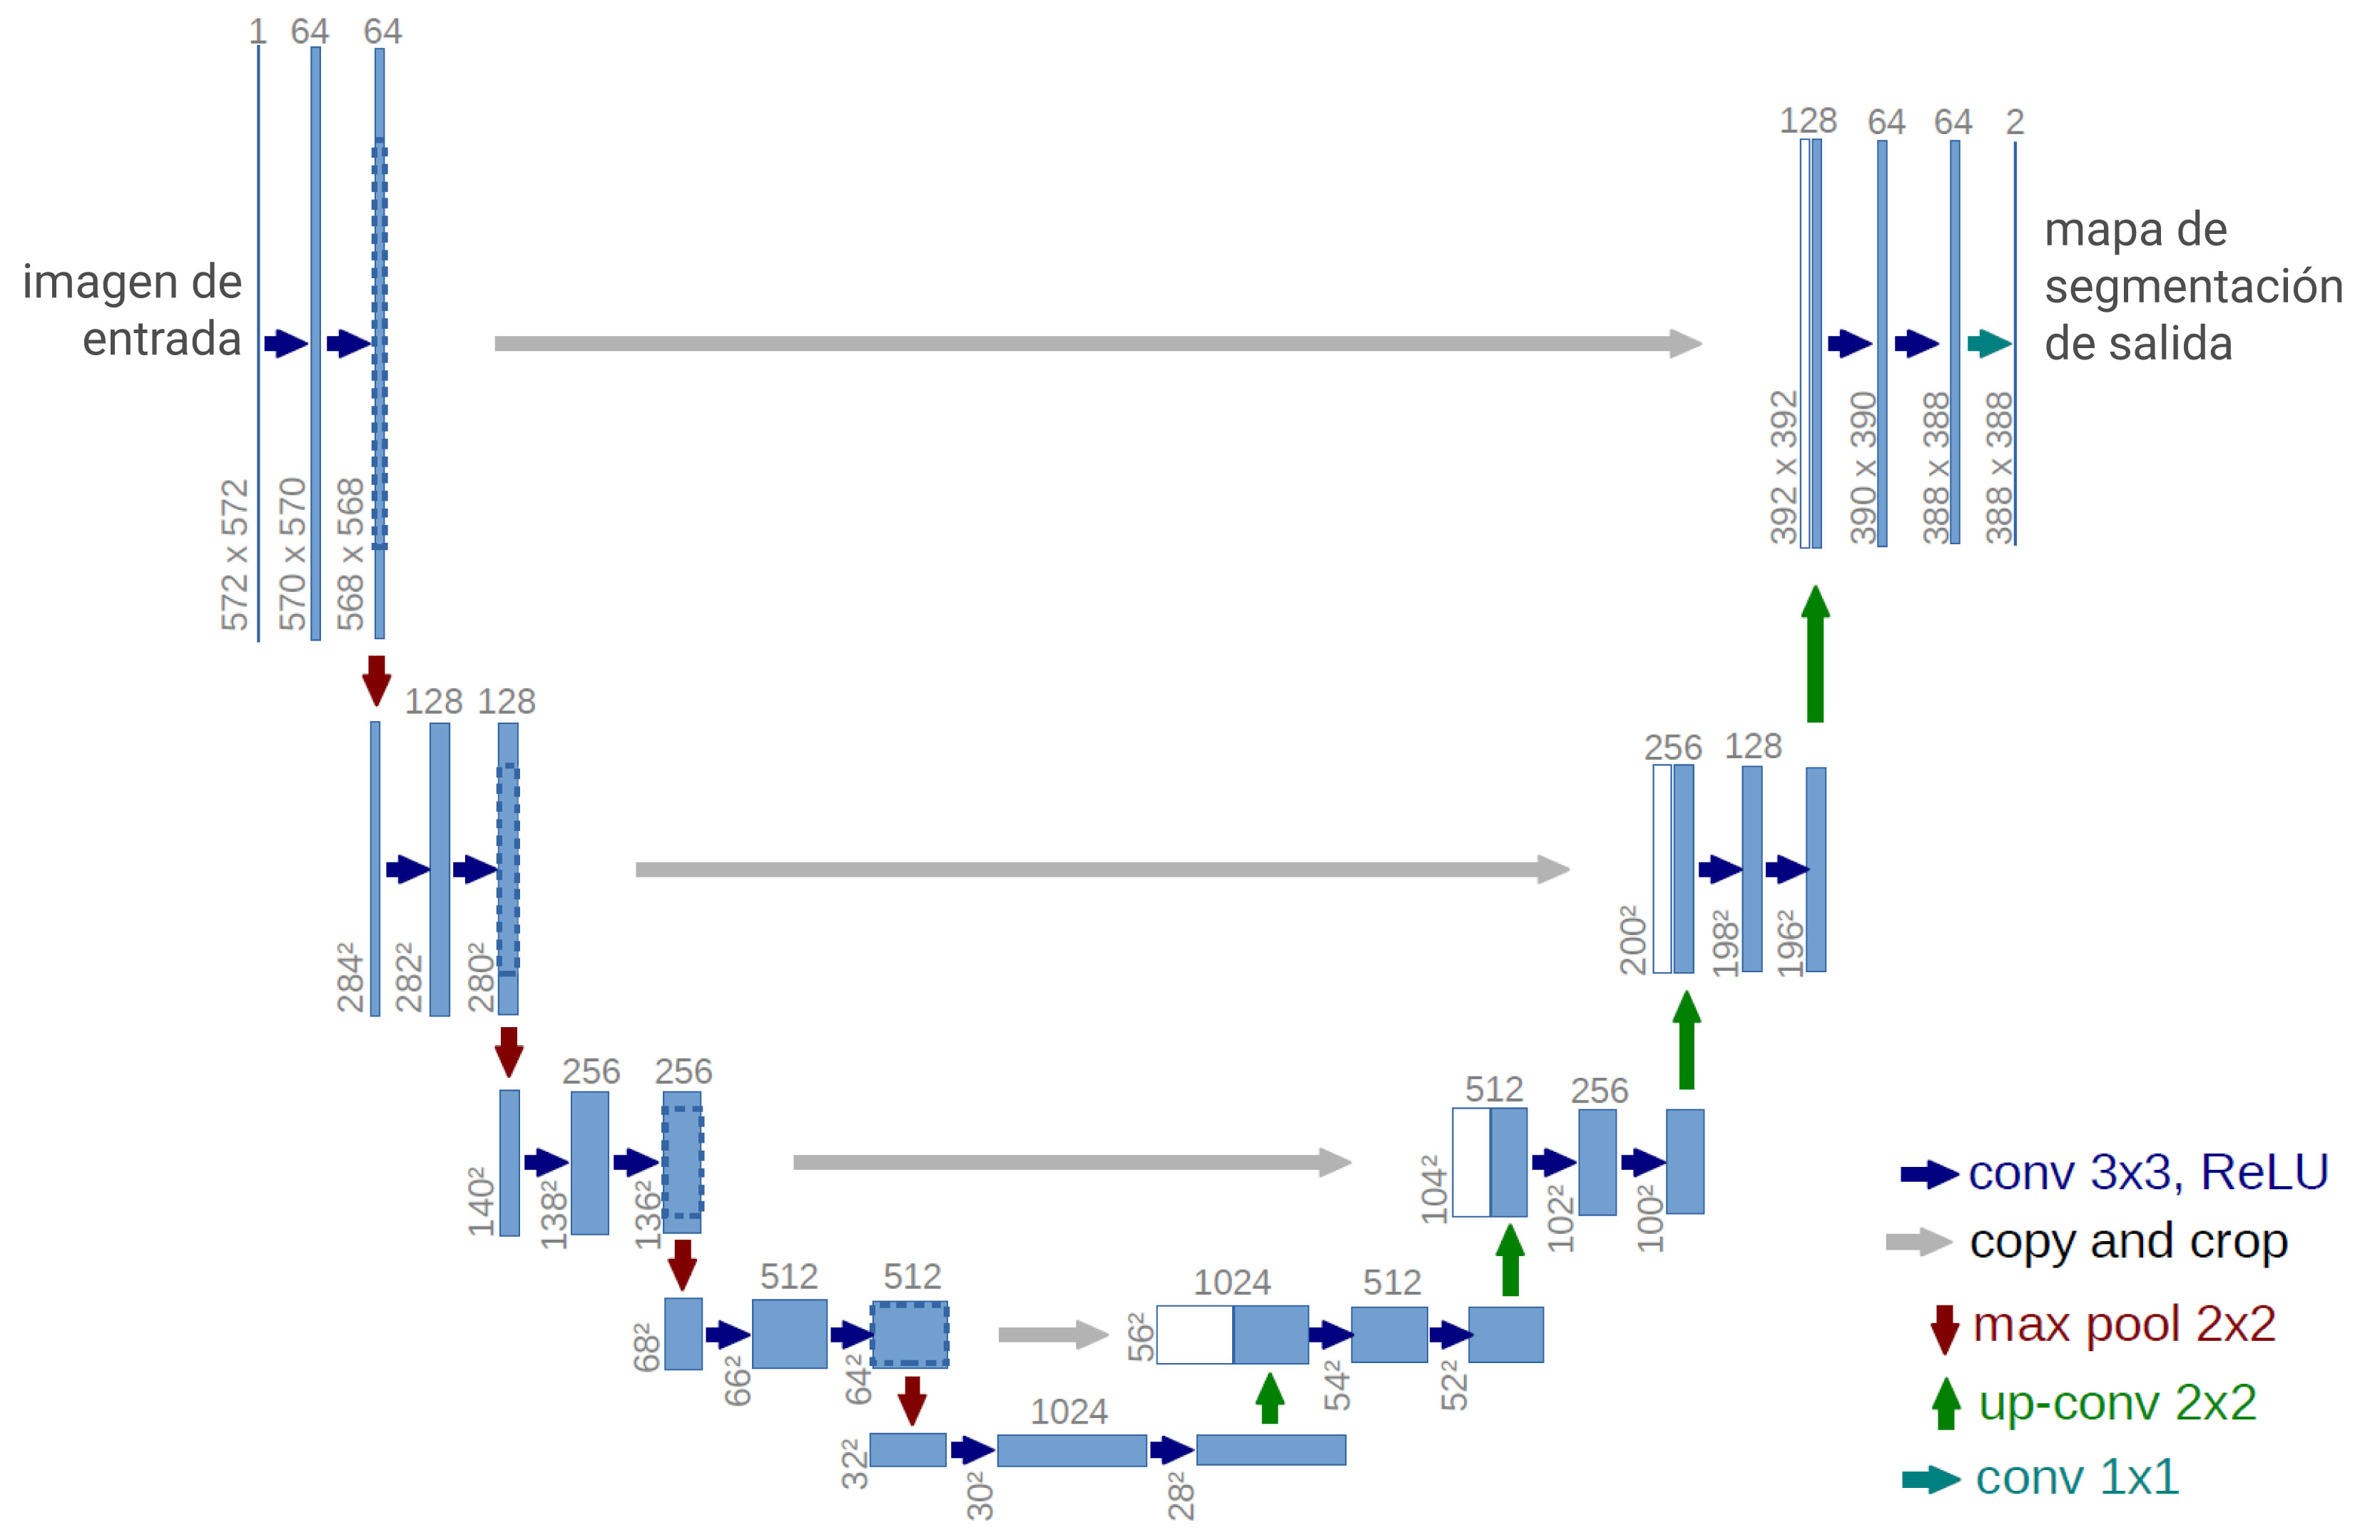
\includegraphics[width=10cm]{./Graphics/unet.png}
	\caption{Arquitectura UNet (ejemplo de 32 $\times$ 32 píxeles en su menor resolución). Cada rectángulo azul corresponde a un mapa de características multicanal. El número de canales se denota en el tope del rectángulo y los tamaños $x-y$ en la esquina inferior derecha. Los rectángulos blancos representan copias de los mapas de características. Las flechas muestras las diferentes operaciones. Tomada de~\cite{ronneberger2015u}.}
	\label{fig:unet}
\end{figure}

La arquitectura, reflejada en la figura \ref{fig:unet}, consta de un camino de contracción (lado izquierdo) para la captura del contexto y otro camino simétrico de expansión (lado derecho) que habilita la localización precisa.

El camino de contracción está formado por la aplicación de repetidas capas convolucionales de 3 $\times$ 3, cada una seguida por una capa \textit{ReLU} (Unidad Lineal Rectificada) y una capa \textit{Max-Pooling} (Operación de Agrupamiento Máximo) de 2 $\times$ 2 para la reducción de resolución de muestreo (\textit{downsampling}). Cada paso en el camino expansivo contiene una ampliación de la resolución (\textit{upsampling}) del mapa de características, una concatenación con su correspondiente mapa de características recortado del primer camino y dos convoluciones de 3 $\times$ 3, seguidas de capas \textit{ReLU}. La última capa usa una convolución 1 $\times$ 1 para obtener la clasificación final de cada píxel dependiendo del número de clases. En total, UNet cuenta con 23 capas convolucionales~\cite{ronneberger2015u}.

\subsubsection{LinkNet}

LinkNet es una arquitectura de RNC utilizada en la segmentación semántica, que predice de forma precisa sin sacrificar el tiempo de procesamiento. Esta arquitectura transfiere información espacial directamente desde el camino de contracción hacia el de expansión en los pasos correspondiente, de esta forma mejora la precisión~\cite{chaurasia2017linknet}.

\begin{figure}[ht]
	\centering
	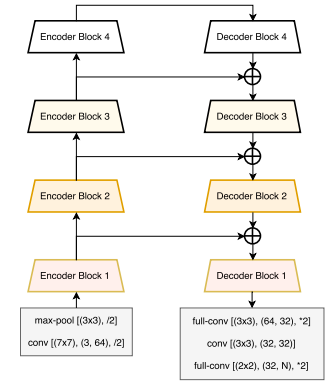
\includegraphics[width=7cm]{./Graphics/linknet.png}
	\caption{Arquitectura LinkNet. Tomada de ~\cite{chaurasia2017linknet}.}
	\label{fig:linknet}
\end{figure}

La arquitectura de LinkNet se presenta en la Figura \ref{fig:linknet}. En la figura, \verb|conv| significa convolución y \verb|full-conv| significa convolución completa. Además, \verb|/2| denota reducción de muestreo por un factor de 2 que se logra al realizar una convolución estriada y \verb|*2| significa aumento de muestreo por un factor de 2. Se utiliza la normalización por lotes (\textit{batch normalization}) entre cada capa convolucional y que es seguida por la no linealidad de \textit{ReLU}. La mitad izquierda de la red que se muestra en la Figura \ref{fig:linknet} es el camino de contracción, mientras que la derecha es el camino de expansión.

\begin{figure}[ht]
	\centering
	\begin{subfigure}
		\centering
		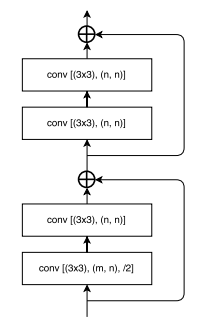
\includegraphics[width=.4\linewidth]{./Graphics/encoder.png}
	\end{subfigure}
	\begin{subfigure}
		\centering
		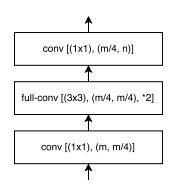
\includegraphics[width=.4\linewidth]{./Graphics/decoder.png}
	\end{subfigure}
	\caption{\textit{Encoder block} (izquierda) y \textit{decoder blocks} (derecha). Tomada de~\cite{chaurasia2017linknet}.}
	\label{fig:blocks}
\end{figure}

El camino de contracción comienza con un bloque inicial que realiza la convolución en la imagen de entrada con un \textit{kernel} de tamaño 7 $\times$ 7 y un paso de 2. Este bloque también realiza una agrupación máxima espacial (\textit{Spatial Max-Pooling}) en un área de 3 $\times$ 3 con un paso de 2. La última parte del camino de contracción consta de bloques residuales y se representan como \textit{encoder blocks}. Las capas dentro de estos \textit{encoder blocks} se muestran en detalle en la Figura \ref{fig:blocks} (izquierda). De igual forma, los detalles de los \textit{decoder blocks} se presentan en la Figura \ref{fig:blocks} (derecha). La principal diferencia entre esta arquitectura con otras es el traspaso de información de los \textit{encoder blocks} hacia los \textit{decoder blocks}, de forma que esta información no tiene que ser aprendida.

\subsection{Evaluación de la segmentación}\label{sec:evalSeg}

Para conocer la calidad de los resultados de un proceso de segmentación, es necesario utilizar alguna medida de evaluación. Existen diferentes medidas para lograr este objetivo. A continuación se presentan los conceptos principales para la evaluación de la calidad de los algoritmos de segmentación.

La segmentación semántica particiona los píxeles en clases, por tanto se puede resumir esta tarea a un problema de clasificación. Para evaluar clasificaciones suele utilizarse el concepto de matriz de confusión.

\begin{definition}
	Se entiende por Matriz de Confusión como una matriz de orden $2$ que cuantifica la frecuencia que cada categoría es bien clasificada o no frente a las otras categorías.
\end{definition}

En el caso de la clasificación binaria la matriz de confusión queda como sigue:

\begin{table}[ht]
	\centering
	\begin{tabular}{|| c || c | c ||}
		\hhline{|=||=|=|}
		
		Real /Predicción & 0 & 1\\ \hhline{||=||=|=||}
		0 & VN & FP\\
		1 & FN & VP \\ \hhline{|=||=|=|}
	\end{tabular}
	\caption{Matriz de confusión}
	\label{tab:conf}
\end{table}

\begin{itemize}
	\item VN representa la cantidad  de los verdaderos negativos: aquellos elementos que pertenecen a la categoría 0 y se predice que pertenecen a la categoría 0.
	\item FP representa la cantidad  de  los falsos positivos: aquellos elementos que pertenecen a la categoría 0 y se predice que pertenecen a la categoría 1.
	\item FN representa la cantidad  de  los falsos negativos: aquellos elementos que pertenecen a la categoría 1 y se predice que pertenecen a la categoría 0.
	\item VP representa la cantidad  de  los verdaderos positivos: aquellos elementos que pertenecen a la categoría 1 y se predice que pertenecen a la categoría 1.
\end{itemize}

Entre las métricas de evaluación más comunes en problemas de clasificación se encuentra:

\begin{definition}
	Precisión (P): medida que cuantifica la fracción de elementos positivos o de categoría 1 que son clasificados correctamente. 
	$$ P = \frac{VP}{FP + VP}$$	
\end{definition}

\begin{definition}
	Recobrado o recall (R): medida que cuantifica la fracción de elementos positivos o de categoría 1 que son clasificados.
	$$ P = \frac{VP}{FN + VP}$$	
\end{definition}

Estas dos medidas son de vital importancia pero por separado no indican la buena o mala calidad de los resultados en la segmentación semántica. En la segmentación no solo interesa cuán precisa es la salida del proceso, sino que también se clasifique la mayor cantidad de elementos de la clase o de categoría 1. Una solución sería clasificar todos los elementos como de categoría 1, lo cual no es una respuesta factible. Por tanto se necesita un equilibrio entre ambas métricas, para lograr un recobrado alto tolerando una pequeña cantidad de falsos positivos.

A continuación se presentan dos de las medidas más utilizadas para evaluar la tarea de segmentación.

\begin{itemize}
	\item \textbf{Índice de similaridad Jaccard (IJ)}: es una métrica que permite cuantificar el solapamiento entre una máscara objetivo y la salida de algún método de segmentación. El valor de $IJ$ cuenta el número de píxeles comunes entre la máscara objetivo y la predicción, dividido por el total de números de píxeles entre las dos máscaras. Se cumple
	\begin{equation}
		\text{IJ} = \frac{VP}{FN + VP + FP},
	\end{equation}
donde $GT$ es medida de verdad o \textit{ground truth} y $P$ es la predicción.
	
	\item \textbf{Índice de similaridad de Dice (F1-Score):} es una medida que armoniza la Precisión ($P$) y el Recobrado ($R$) de los resultados de la segmentación. El F1-Score toma un valor alto cuando $P$ y $R$ tiene valores altos, por lo que la determinación del valor máximo para F1-Score puede interpretarse como un esfuerzo por encontrar el mejor compromiso entre $P$ y $R$. Se cumple
	\begin{equation}
		\text{F1-Score} = \frac{2PR}{P + R}.
	\end{equation}
\end{itemize}

\section{Reconstrucción 3D a través de Cámaras de profundidad (RGB-D)}\label{section:rec3d}

La \textit{Reconstrucción 3D} es el proceso de generar un modelo computacional de tres dimensiones en forma de malla poligonal que refleja la apariencia y forma de una escena real con datos capturados por sensores. Una de las fuentes adquisitivas de estos datos son los sensores RGB-D integrados a las cámaras de profundidad.

Desde sus inicios el potencial de las cámaras RGB-D fue rápidamente reconocido en el campo de la visión computacional. No solo están disponibles a un bajo precio, además sus sensores capturan imágenes de color y profundidad. Dichas características las posicionan incluso por encima de costosos sistemas de escaneo 3D en determinadas tareas.

En el ámbito de la reconstrucción 3D se han diseñado numerosos e innovadores algoritmos a partir de los cuales se obtienen modelos computacionales que representan escenas estáticas, dinámicas y otros que incluso capturan propiedades adicionales. Esta tarea se puede realizar de dos formas:
\begin{itemize}
	\item Tiempo Real: donde se reconstruye  a medida que se capturan las imágenes,
	\item A posteriori: donde se adquiere primeramente el conjunto de imágenes y luego se pasa al proceso de reconstrucción.
\end{itemize}

Es importante tener en cuenta estos aspectos para seleccionar el algoritmo más adecuado a la situación y condiciones ambientales del problema en cuestión. En la figura \ref{fig:r3d} se muestra el flujo de procesamiento típico de un sistema de reconstrucción RGB-D para este tipo de escenarios.

\begin{figure}[ht]
	\centering
	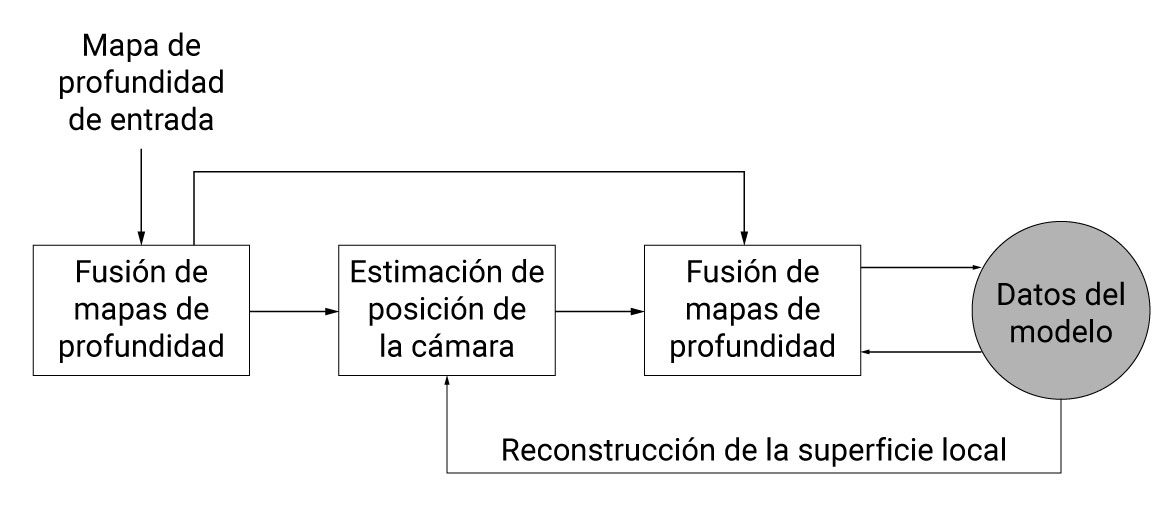
\includegraphics[width=10cm]{./Graphics/r3d.png}
	\caption{Muestra del flujo típico de un sistema de reconstrucción RGB-D: primero, la imagen de entrada preprocesada se alinea respecto a la superfice de reconstrucción actual; segundo, dada la estimación de la posición de la cámara, la entrada es integrada/fusionada en el actual modelo 3D de la reconstrucción~\cite{zollhofer2018state}.}
	\label{fig:r3d}
\end{figure}

En la próxima subsección se profundiza en un Sistema de Reconstrucción 3D a posteriori, que consecuentemente captura solo la naturaleza de escenas estáticas. Por otra parte, permite realizar optimizaciones que no son factibles de ejecutar en tiempo real y puede resultar en mayor precisión de las estimaciones. Antes se presentan algunas definiciones necesarias para su comprensión.

\begin{definition}
	El Registro o Alineación entre dos imágenes (entre dos nubes de puntos) $P_1$ y $P_2$ es el proceso de encontrar una transformación espacial $M$, que minimice cierta función de distancia definida entre $P_1$ y $P_2$.
\end{definition}

\begin{definition}
	La Odometría Visual se define como el conjunto de algoritmos que ayudan a estimar el movimiento, tomando información de las imágenes capturadas por sensores.
\end{definition}

\begin{definition}
	La Función Signada de Distancia Truncada (TSDF, por sus siglas en inglés, de Truncated Signed Distance Function) es una representación volumétrica 3D de una escena donde a cada voxel~\footnote{Voxel, unidad de información gráfica que define un punto en un espacio de tres dimensiones.} almacena la distancia a la superficie más cercana~\cite{curless1996volumetric}
\end{definition}


\begin{definition}
	Una Malla Poligonal es una estructura de datos que consta de una colección de vértices, caras y aristas. Es utilizada para describir objetos u escenas mediante modelos poliédricos 3D. Las caras usualmente consisten en triángulos (mallas triangulares), aunque es un factor que puede variar.
\end{definition}


\subsection{Método de Reconstrucción 3D}\label{section:rec3dmet}

El flujo de trabajo descrito en esta subsección es un sistema de reconstrucción de escenas completas, basado en el artículo~\cite{choi2015robust} y adoptando ideas introducidas en~\cite{park2017colored} para lograr mejores resultados. Fue desarrollado por el equipo de la biblioteca \textit{Open3D}~\cite{zhou2018open3d}, haciendo uso de múltiples algoritmos implementados en la misma. Toma como entrada la secuencia $\hat{S}$ de imágenes RGB-D sincronizadas y alineadas, junto a la matriz intrínseca de la cámara, la cual forma parte de los parámetros entrantes de muchos algoritmos internos del sistema. Procede de la siguiente forma:

\begin{enumerate}
	\item \textbf{Construcción de Fragmentos:} Las imágenes individuales tienen ruido y son incompletas. Por tanto, para manejar información más confiable de las superficies geométricas locales, se divide $\hat{S}$ en segmentos de $k$-cuadros (\textit{$k$-frames}). A todos los pares que se forman en una subsecuencia se les aplica Odometría RGB-D para estimar su alineación o registro. Se crea un grafo de posiciones de todas las imágenes del fragmento cuyos nodos representan una imagen RGB-D  y su posición (la primera aproximación de esta posición es la correspondiente a la alineación con su imagen antecedente en la secuencia), que transforma la geometría al espacio global del fragmento; las aristas contienen la información de la odometría entre los pares con registro satisfactorio. A las posiciones del grafo se les aplica optimización con el algoritmo Levenberg-Marquardt~\cite{more1978levenberg}. Por último, cada secuencia se integra en un volumen TSDF. La malla que se extrae de cada volumen representa un fragmento a colores.
	
	\item \textbf{Registro Geométrico:} Una vez creados los fragmentos de la escena el próximo paso es alinearlos en un espacio global. Primeramente, se registran los pares de  fragmentos para estimar un alianeación básica. Si son vecinos se utiliza el método ICP y en otro caso RANSAC (\textit{RANdom SAmple Consensus}) o Registro Global Rápido. Se procede a construir el grafo de posiciones de los fragmentos y se le aplica el mismo método de optimización del paso anterior.
	
	\item \textbf{Refinamiento del Registro e Integración de la Escena:} Para lograr un refinamiento de las alineaciones se aplica el algoritmo ICP sobre los pares detectados en registro geométrico; se crea un nuevo grafo de posiciones con los registros refinados; y se ejecuta la optimización en dichas posiciones como previamente mencionado en 1. El último paso del sistema es la integración de todas las imágenes RGB-D en un solo volumen TSDF y la extracción de la malla resultante.
\end{enumerate}

\begin{figure}[ht]
	\centering
	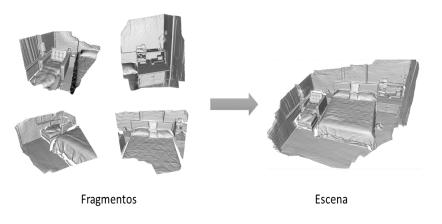
\includegraphics[width=10cm]{./Graphics/algo3d.png}
	\caption{Ejemplo de resultados del algoritmo de reconstrucción. A la derecha se muestra el conjunto de fragmentos de la escena y a la izquierda la reconstrucción final formada a partir de los fragmentos. El ejemplo muestra la escena sin colores.}
\end{figure}

\section{Estimadores de perímetro, área y volumen en mallas poligonales}\label{section:measure}

El diseño de estimadores espaciales como son el perímetro, área y volumen en mallas poligonales constituye otra de las tareas trascendentales del trabajo. Antes de explicar el diseño de los estimadores se presentan algunos conceptos importantes en el diseño.

\begin{definition}
	Se define como envoltura convexa de un conjunto de puntos $X$ de dimensión $n$ como el mínimo de todos los conjuntos convexos que contienen a $X$. 
\end{definition}

La envoltura convexa de un conjunto $X = \{x_1, x_2, \ldots, x_k\}$ está dada por la expresión:
$$ C(X) = \bigg\{\sum_{i = 1}^{k} \alpha_i x_i | x_i \in X, \alpha_i \in \mathbb{R}, \alpha_i \geq 0, \sum_{i = 1}^{k} \alpha_i = 1\bigg\}.$$

La computación de la envoltura convexa de una nube finita de puntos, especialmente en el plano, ha sido exhaustivamente estudiada y tiene aplicaciones, como por ejemplo, en el procesado de imágenes y en localización. Existen muchos métodos para el cálculo de la envoltura convexa, en el trabajo se utiliza el algoritmo \textit{Quick Hull}~\cite{barber1996quickhull} implementado en \textit{Open3d}~\cite{zhou2018open3d}.

\begin{definition}
	La Triangulación de Delaunay para un conjunto $P$ de puntos de $n$ dimensiones es una triangulación $DT$ de $P$ tal que ningún punto en $P$ está dentro de la circun-hiperesfera de ningún $n$-simplex~\footnote{Un simplex es una generalización de la noción de triángulo o tetraedro a dimensiones arbitrarias.} en $DT$.
\end{definition}

La Triangulación de Delaunay para un conjunto de puntos $P$ no es única, en el caso de que la dimensión espacial de los puntos de $P$ sea tres, la triangulación produce pirámides triangulares. El algoritmo utilizado en la implementación de \textit{Scipy}~\cite{virtanen2020scipy} es el algoritmo \textit{Quick Hull}~\cite{barber1996quickhull}.

\subsection{Perímetro}

El perímetro de una malla poligonal que representa una úlcera se define como la longitud de los lados de la figura en 2D de la úlcera. Para la estimación del perímetro se procede:

\begin{enumerate}
	\item \textbf{Proyección al plano:} Se concibe como la etapa en la que se proyecta la malla poligonal en tres dimensiones en una figura plana. La nube de puntos $P$ que conforma la malla está compuesta por puntos de tres componentes $p_i = (x_i, y_i, z_i)$. Para la proyección se transforma la nube de puntos $P$ en $P_{2D}$ la cual cumple que $\forall p_i \in P_{2D}: p_i = (x_i, y_i, 0)$.
	
	\item \textbf{Envoltura convexa de $P_{2D}$:} Los puntos $p_{qhull}$ se definen como los vértices de la envoltura convexa de $P_{2D}$. Se calcula la envoltura convexa de $P_{2D}$ y se toman los $p_{qhull}$ y las aristas.
	
	\item \textbf{Sumatoria de la distancia entre puntos $p_{qhull}$:} Luego, el perímetro total de la úlcera no es más que la suma de la longitud de las aristas o la distancia entre los $p_{qhull}$ adyacentes. Para calcular la longitud se utiliza la distancia euclidiana.
	
\end{enumerate}

\subsection{Área}

El área de una figura geométrica hace referencia a la superficie de la misma, es decir, al espacio que queda encerrado en los límites de la misma. La estimación del área de una malla poligonal se define como la sumatoria del área de todas las caras triangulares que conforman la malla. Para el cálculo del área de los triángulos se utiliza la fórmula de Herón 
$$A = \sqrt{s(s-a)(s-b)(s-c)}$$
donde $s = \frac{P_t}{2}$ y $P_t$ es el perímetro de la cara triangular. Por tanto, el área de la malla poligonal $A_M$ con $k$ caras se calcula como
\begin{equation}
	A_M = \sum_{i = 0}^{k} A_k
\end{equation}
donde $A_k$ es el área de la cara $k$-ésima de la malla poligonal.

\subsection{Volumen}

El volumen es una magnitud métrica de tipo escalar asociada a la extensión en tres dimensiones de una región del espacio. Las úlceras se pueden definir como cavidades en una superficie, por tanto el volumen de una úlcera no es más que el volumen de la cavidad.

La estimación del volumen de una úlcera en este caso particular se concibe como un proceso de varias etapas.  Como primer paso es necesario aproximar la superficie que cubre la cavidad, esta superficie será llamada tapa $T_U$ de la úlcera con malla $U$. Luego, se forma la malla compuesta de $C = T_U + U$ y se calcula el volumen de esta malla, realizando una triangulación de Delaunay y sumando el volumen de las pirámides resultantes. Por tanto el volumen de la malla $C$ es
\begin{equation}
	V_C = \sum_{i = 0}^{k} V_{\pi_i}
\end{equation}
donde se cumple que: 
\begin{itemize}
	\item $C$ es la malla compuesta por $T_U$ y $U$.
	\item $\Pi$ es el conjunto de pirámides resultantes de la triangulación de Delaunay de $C$. Luego, $\pi_i \in \Pi: 1 \leq i \leq k = |\Pi|$
	\item $V_{\pi_i}$ es el volumen de la pirámide triangular $i$-ésima cuya fórmula es $V_{\pi_i} = \frac{1}{3}A_t * h$, con $A_t$ es el área de una de las caras de la pirámide denotada $t$ y $h$ es la altura de la pirámide calculada como la distancia desde el plano formado por $t$ hasta el vértice sobrante de $\pi_i$.
\end{itemize}

En este capítulo se han resumido los conceptos matemáticos y computacionales esenciales de los métodos aplicados para la obtención del sistema de medición 3D de UPD que se tiene como objetivo. En el próximo capítulo se presenta el sistema que tiene como fundamento la reconstrucción 3D no invasiva de la úlcera.


